\section{Operating Principles}

\subsection{Concept of Autonomy and Safety}

To make a significant contribution to the crypto economy's freedom 
and independence, a new secure and autonomous stablecoin is required 
to minimize the risks associated with centralization and crypto 
market volatility.

Existing stablecoins are susceptible to the following risks due to their 
strong connection to the traditional financial system, which is unpredictable:

\begin{enumerate}
\item Risks due to centralization:
	\begin{enumerate}
		\item Stable tokens can be banned/frozen, or the address can be blacklisted by authorized actors.
    \item The creators of stablecoins can be influenced using legal or other means.
    \item Some functions of stablecoin tokens might stop working if the project
    team stops supporting the project, such as collateral re-balancing or 
    mint/redeem for centralized stables.
    \item Collateral containing cash/treasuries or other stablecoins that include 
    cash/treasuries can collapse due to various situations in the banking system 
    or financial regulation issues.
  \end{enumerate}
\item Risks due to crypto market unpredictability and volatility:
	\begin{enumerate}
    \item A stablecoin might collapse if its internal business model operates incorrectly. 
    Dependency on the internal business model makes its behavior much more unpredictable, for example:
    \begin{itemize}
      \item For continuous support, a stablecoin project team needs funds. Thus, it needs 
      revenue generation in some form. For USDT/USDC and other stablecoins backed 
      by cash/treasures, it is the interest returned from deposits and treasury bond yields. 
      For DAI and other stablecoins backed by crypto assets, the revenue is fees and commissions 
      from lending and borrowing.
    \end{itemize}
    \item Collateral containing crypto assets can depreciate in value due to a decline 
    in the crypto market. If the crypto market is down significantly, it can unpeg 
    a crypto-backed stablecoin from USD.
  \end{enumerate}
\end{enumerate}



The USSD stablecoin aims to avoid the risks associated with existing stablecoins 
by implementing the following features:
\begin{enumerate}
  \item No methods for freezing, blacklisting, banning or pausing transfers are 
  implemented in the smart-contract. The goal is to make the USSD stablecoin completely unstoppable.
  \item USSD is a non-profit, long-term project that exists autonomously without any 
  connection to physical entities. Only code is used, making it non-biased and secure.
  \item The architecture of the USSD stablecoin is designed to be autonomous.
  \item Since the USSD protocol operates independently of any business model, it 
  eliminates the risks associated with the bankruptcy of such models.
  \item USSD's collateral structure is designed to maintain a collateral to capitalization 
  ratio of more than 10x.
\end{enumerate}

\begin{table}
\caption{Comparison of stablecoin features}
\raggedleft
\begin{tabular}{|>{\hspace{0pt}}m{0.156\linewidth}|>{\hspace{0pt}}m{0.158\linewidth}|>{\hspace{0pt}}m{0.175\linewidth}|>{\hspace{0pt}}m{0.175\linewidth}|>{\hspace{0pt}}m{0.14\linewidth}|>{\hspace{0pt}}m{0.133\linewidth}|} 
\hline
\par{}                                   & \textbf{USDT}                                                                             & \textbf{USDC}                                                             & \textbf{USDP}                                                       & \textbf{DAI}                                                              & \textbf{USSD}                                                     \\ 
\hline
Transparency                             & {\cellcolor[rgb]{1,0.843,0.843}}based on auditor reports\textsuperscript{1} & {\cellcolor[rgb]{1,0.843,0.843}}by paper proof\textsuperscript{2} & {\cellcolor[rgb]{1,0.843,0.843}}by paper proof \textsuperscript{3} & {\cellcolor[rgb]{1,1,0.843}}partially by code\textsuperscript{4} & {\cellcolor[rgb]{0.867,0.91,0.796}}by code            \\ 
\hline
Source of collateral                     & {\cellcolor[rgb]{1,0.843,0.843}}short-term US treasuries, cash, etc.                          & {\cellcolor[rgb]{1,0.843,0.843}}short-term US treasuries, cash in US banks     & {\cellcolor[rgb]{1,0.843,0.843}}short-term US treasuries, cash in US banks      & {\cellcolor[rgb]{1,1,0.843}}ERC20 (ETH, wBTC), Real World Assets token funds, USDC         & {\cellcolor[rgb]{0.867,0.91,0.796}}crypto-backed  \\ 
\hline
Crypto collateral ratio                        & {\cellcolor[rgb]{1,0.847,0.808}}2\%                                             & {\cellcolor[rgb]{1,0.847,0.808}}0\%                                         & {\cellcolor[rgb]{1,0.847,0.808}}0\%                                          & {\cellcolor[rgb]{0.867,0.91,0.796}}{\raise.17ex\hbox{$\scriptstyle\sim$}}~150\% \textsuperscript{5}                & {\cellcolor[rgb]{0.867,0.91,0.796}}{\raise.17ex\hbox{$\scriptstyle\sim$}}~500\% (projected)      \\ 
\hline
Full collateral ratio                        & {\cellcolor[rgb]{1,0.847,0.808}}claimed 100\%                                             & {\cellcolor[rgb]{1,1,0.843}}claimed 100\%                                         & {\cellcolor[rgb]{1,1,0.843}}claimed 100\%                                          & {\cellcolor[rgb]{0.867,0.91,0.796}}{\raise.17ex\hbox{$\scriptstyle\sim$}}claimed ~278\%                 & {\cellcolor[rgb]{0.867,0.91,0.796}}{\raise.17ex\hbox{$\scriptstyle\sim$}}~500\% (projected)      \\ 
\hline
Regulatory status                         & {\cellcolor[rgb]{1,1,0.843}}Hong Kong entity                                              & {\cellcolor[rgb]{1,1,0.843}}US entity                                     & {\cellcolor[rgb]{1,0.847,0.808}}several entities                           & {\cellcolor[rgb]{1,1,0.843}}US entity                                     & {\cellcolor[rgb]{0.867,0.91,0.796}}no entity                      \\ 
\hline
Centralization level of token management & {\cellcolor[rgb]{1,0.847,0.808}}team can freeze tokens, manage collateral                                     & {\cellcolor[rgb]{1,0.847,0.808}}team can freeze tokens, manage collateral                     & {\cellcolor[rgb]{1,0.847,0.808}}team can freeze tokens, manage collateral                      & {\cellcolor[rgb]{1,1,0.843}}DAO can manage collateral                     & {\cellcolor[rgb]{0.867,0.91,0.796}}no-one can freeze tokens, no-one can manage collateral        \\ 
\hline
Project Management                       & {\cellcolor[rgb]{1,0.847,0.808}}centralized, manual                                       & {\cellcolor[rgb]{1,0.847,0.808}}centralized, manual                       & {\cellcolor[rgb]{1,0.847,0.808}}centralized, manual                        & {\cellcolor[rgb]{1,1,0.843}}DAO managed, manual                           & {\cellcolor[rgb]{0.867,0.91,0.796}}autonomous                     \\ 
\hline
Business model                           & {\cellcolor[rgb]{1,1,0.843}}US treasuries yield                                                  & {\cellcolor[rgb]{1,1,0.843}}US treasuries yield                                  & {\cellcolor[rgb]{1,1,0.843}}US treasuries yield                                   & {\cellcolor[rgb]{1,0.847,0.808}}RWA token funds partnership \%, DAI borrowing interest                         & {\cellcolor[rgb]{0.867,0.91,0.796}}non-profit, everyone has equal opportunities                     \\
\hline
\end{tabular}
\end{table}

\nopagebreak

\addtocounter{footnote}{1}
\footnotetext{https://tether.to/en/transparency/\#reports}
\addtocounter{footnote}{1}
\footnotetext{https://www.circle.com/en/usdc\#transparency}
\addtocounter{footnote}{1}
\footnotetext{https://paxos.com/busd-transparency/}
\addtocounter{footnote}{1}
\footnotetext{MakerDAO's protocol details are accessible via a provided link, yet a significant portion of DAI's collateral, approximately 50-60\%, is held in RWA token funds. The transparency of these funds is maintained through regular reporting.}
\addtocounter{footnote}{1}
\footnotetext{https://daistats.com}


Stablecoins with the largest market capitalization (like USDT / USDC / BUSD / USDP and others) are 
backed by dollar-evaluated collateral with a 1-to-1 ratio. Issuers of such stablecoins 
provide documents that are issued by trusted authorities (auditors). Nevertheless, we consider 
these proofs as paper-proof that contains risks due to their centralized nature, which could 
be affected by corruption, human mistakes, and political influence.

DAI's collateral (crypto assets) is evaluated at a ~278\% ratio to its market capitalization. 
Nevertheless, DAI stablecoin collateral has some notable nuances that bring risks to it (and 
some of them have already been realized):
\begin{itemize}
  \item DAI's collateral contains a major share of RWA tokens and USDC stablecoin (aprroximately 60\% of DAI's capitalization in February 2024), which makes it a cash/US treasuries-backed coin and is regulated by US financial authorities. This means collateral risks of the USDC are also valid for DAI (in March of 2023, DAI depegged from USD because USDC depegged too due to a bank issue, luckily the situation recovered later).
  \item USDC (a part of DAI's collateral) and some other stablecoins have an option of freezing funds (which makes them insecure).
  \item Both DAI and USDC have legal entities in the US and are obliged to comply with all regulatory requirements, making them susceptible to influence.
  \item DAI contains a lending/borrowing protocol as a business model to support its existence, which makes the whole system more complicated, fragile, and dependent on the results of this business operating.
\end{itemize}

\subsection{USSD v2 Architecture}

The USSD stablecoin is composed of three elements: collateral, insurance capital, and a reward staking mechanism. 
\begin{enumerate}
    \item The collateral is a standalone, immutable smart-contract capable of minting and redeeming USSD against BSC-USD, wBTC, and wETH, with no external access permitted. 
    \item The insurance capital serves as a supplemental collateral pool, activated to bolster the main collateral in events of undercollateralization. It is funded by insurance providers who lock in assets (wBGL) permanently and, in exchange, receive ICT tokens, generating ongoing revenue for them. 
    \item Finally, the reward staker is a smart-contract that allows USSD and ICT token holders to stake their tokens, earning interest from the increasing value of the collateral.
\end{enumerate}

\centerline{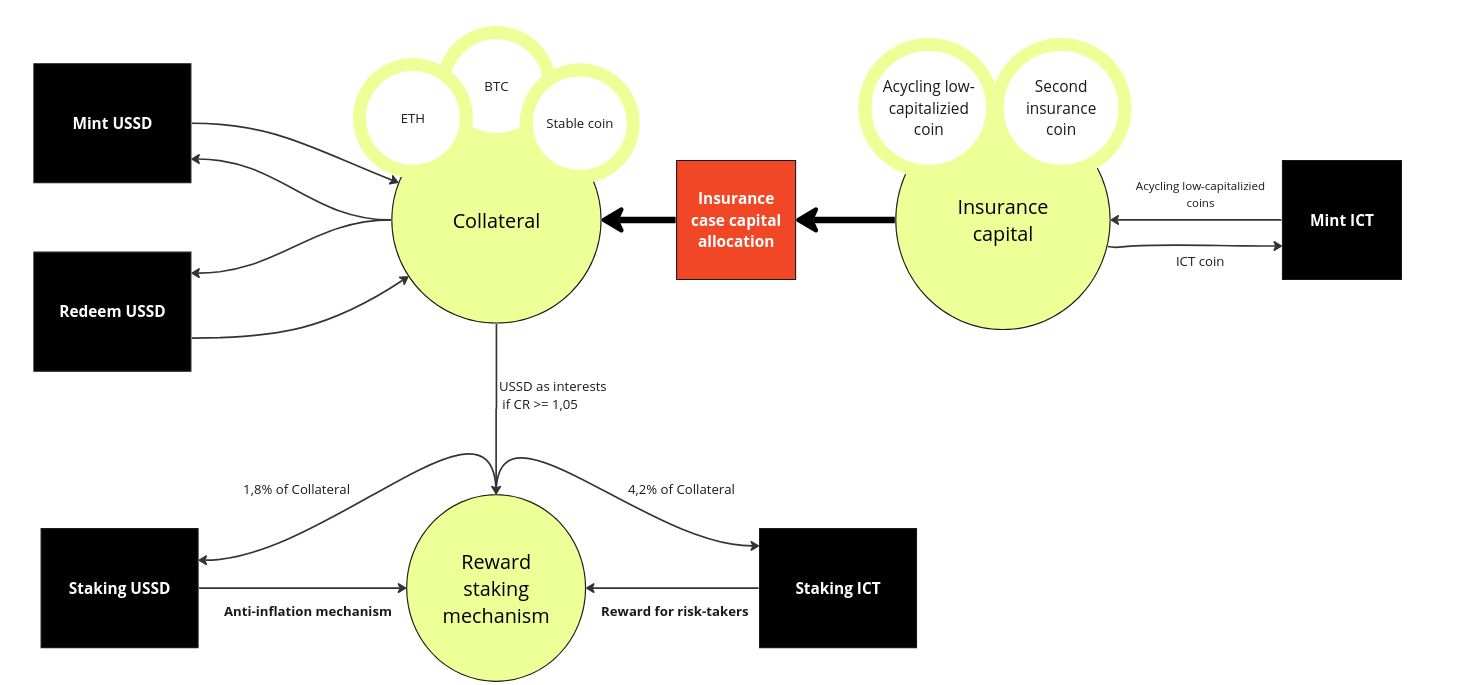
\includegraphics[scale=0.45]{image01.png}}

\subsection{Collateral structure}

The ideal crypto collateral structure should be robust enough to maintain a collateral factor of over 100\% even in harsh scenarios, such as an overall crypto market downturn, a 70-90\% depreciation of BTC/ETH, or even the complete depreciation of one of the crypto assets included as collateral. Due to the high volatility nature of crypto, we have decided to form a collateral structure that will:
\begin{enumerate}
    \item Diversify using the most common and trusted crypto assets, namely BTC and ETH.
    \item Include existing stablecoin (BSC-USD) as part of the collateral to enhance usability and liquidity in USSD stablecoin. Users will be able to redeem BSC-USD in exchange for USSD at any time. 
    \item Create an insurance fund using acyclical coin to safeguard against declining collateral ratios. Unlike cyclical assets that fluctuate with economic conditions, acyclical assets maintain their value and performance independent of the broader economic environment.
    \item Include proportional redeem (details described below).
\end{enumerate}

For strategies combating inflation, increasing the collateral ratio, and fostering project development, it's essential to accumulate or have a growth factor in assets. To maintain simplicity in the model, the only feasible option for a growth factor is its collateral.

Among the most capitalized digital assets in the crypto space, BTC and ETH stand out due to their deflationary mechanisms. Consequently, these assets have been chosen as the primary collateral elements.

\centerline{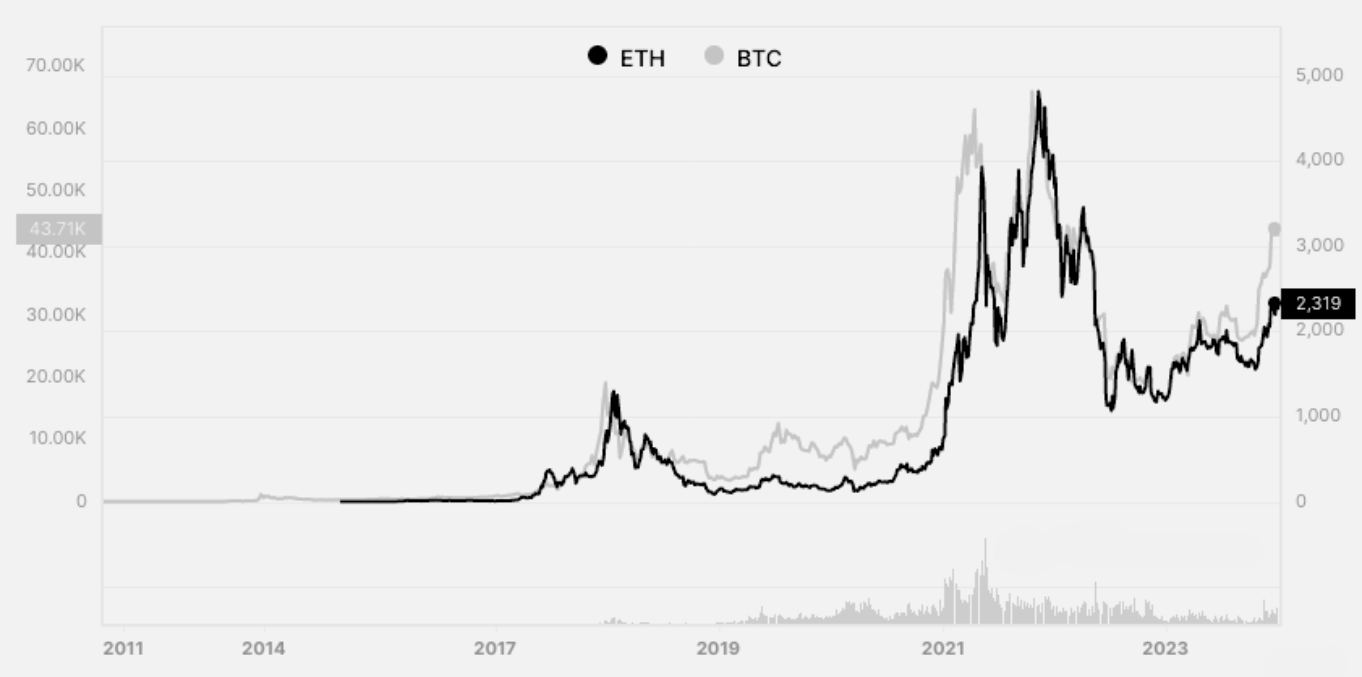
\includegraphics[scale=0.35]{image02.png}}

To make the collateral less volatile and make redeem operation more convenient, it's a good idea to include a small amount of another stablecoin, acting as a hot reserve. The USSD development team chose a stable coin based on specific criteria, prioritizing:

\begin{itemize}
	\item High market capitalization
	\item Wide distribution among holders
	\item Minimal decentralization
\end{itemize}

To ensure room for collateral growth, a portion of 5-15\% from the total USSD balance is set aside for this stablecoin. There are various candidates to be used as stablecoin component, e.g. DAI.

Additionally, it's important to mention that for certain networks (L1 and L2), wrapped versions of assets are used when using the original versions is not possible. The same criteria used for stablecoin apply to the wrapped versions of BTC and ETH.

\subsection{Timing}

The period from 2022 to 2024 is regarded as a "crypto-fall" or "crypto-winter" time, during which the valuations of most crypto assets are low. Hopefully, this period will end soon, and the entire crypto market capitalization will increase by 3-5 times or more, as it has happened several times before. To achieve a high overcollateralization ratio, the USSD stablecoin was created during this time.

\subsection{Cryptomarket stabilization mechanism}

Bitcoin follows a cycle of ups and downs, especially tied to its halving events. Looking at the chart, it's evident that shortly after Bitcoin's halving, its price begins to rise.

\centerline{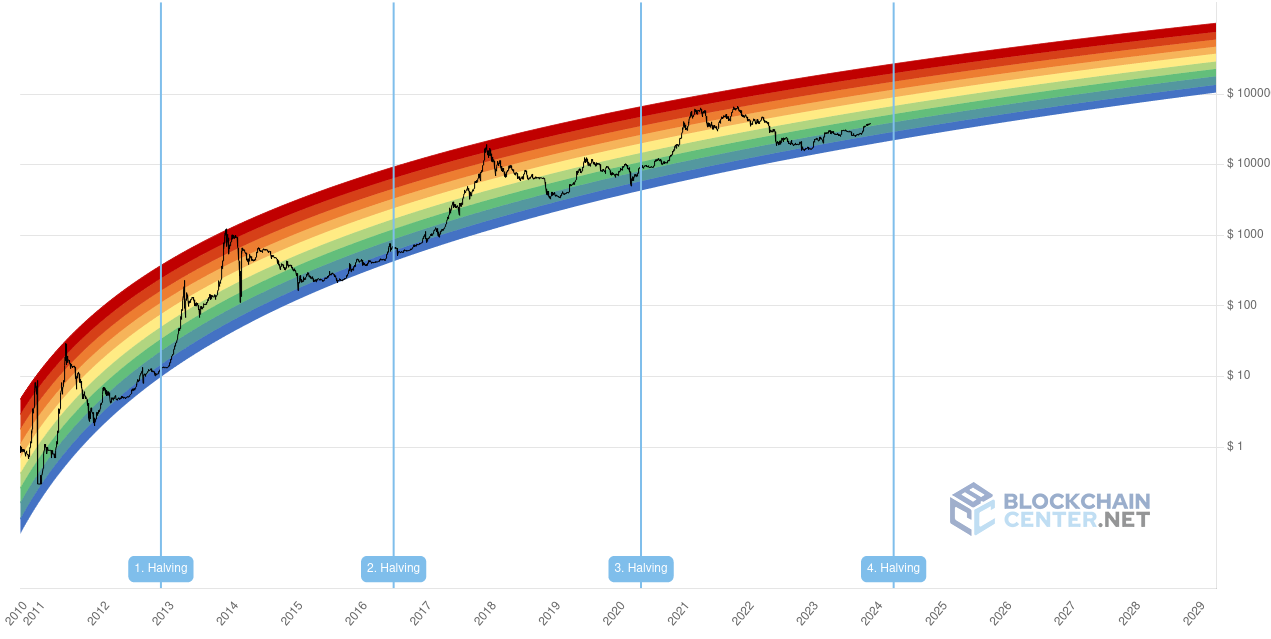
\includegraphics[scale=0.32]{image03.png}}

Halving can be roughly divided into three equal phases after halving, each lasting about one year. Here's a general strategy for collateral accumulation during these phases:

\begin{itemize}
	\item First Phase (First year after halving): Bitcoin (BTC) is growing. It is reasonable to accumulate BTC and ETH in the collateral.
	\item Second Phase (Second year after halving): BTC is at its high levels. It is reasonable to stop accumulating BTC and ETH and focus on accumulating only stable coins.
	\item Third Phase (Third and fourth year after halving): BTC is at its local minimums. It is reasonable to accumulate BTC and ETH in the collateral
\end{itemize}

Very approximately, minting USSD for BTC and ETH is possible in the first, third, and fourth periods. In the second period, it’s possible to mint USSD only for Stable Coin (BSC-USD in USSD v2 bep20).

\subsection{Mint and redeem feature}

The minting and redeem mechanism involves users exchanging crypto assets, such as BSC-USD, WBTC, or WETH for USSD and vice versa.

Users can mint USSD for stablecoin, for WBTC/WETH collateral, or both. Following rules are applied:



\begin{itemize}
   \item During "Crypto Summer" phase of BTC cycle, as WBTC/WETH prices are supposedly at their cycle peak values, mint is allowed only for stablecoin;
   \item If stablecoin collateral component is less than 5\% of USSD's supply, mint is also forced for stablecoin to have it as a reserve for redeem operations (and stablecoin mint is allowed up to 15\% of USSD's supply, or always during "Crypto Summer" mentioned above);
   \item In other cases, WBTC and WETH are accepted as collateral provided to mint USSD.
\end{itemize}

If a user offers assets addresses in mint function that do not fit the criteria, the transaction will be reverted, and the user will pay gas for this unsuccessful transaction if submitted. Any assets directly sent to USSD contract will be stuck on the contract indefinitely (and in case of WBTC, WETH or supported stablecoin would be counted as part of collateral).

\centerline{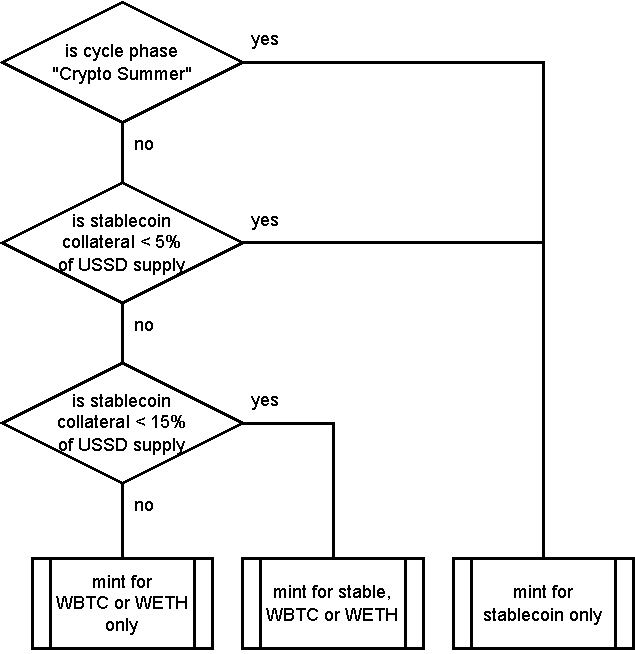
\includegraphics[scale=0.8]{image_mint.pdf}}

Users can redeem USSD (burning USSD and getting collateral assets) following these rules:

\begin{itemize}
	\item If there is stablecoin present as collateral on the USSD contract balance, it would be returned at 1-to-1 ratio for USSD provided;
	\item Secondly, the user will receive WBTC for USSD according to the current market price taken from ChainLink;
	\item Thirdly, the user will receive WETH for USSD according to the current market price taken from ChainLink.
\end{itemize}

This order is designed to decrease the changing levels of core assets in the collateral.

\subsection{Insurance capital}

Cryptocurrency markets can be very unpredictable, and there's a chance that the value of the collateral might go down for a while. To maintain a high over-collateralization ratio, we introduced insurance capital, which includes crypto assets. This capital will be used if there's under-collateralization.

Following criteria were set for selecting assets to be included in the collateral.

\begin{itemize}
	\item The price of this asset shouldn't be closely connected with collateral assets like BTC and ETH;
	\item It should be decentralized;
	\item It should have a balanced deflationary mechanism;
	\item Its level of capitalization should be low at the time of USSD deployment.
\end{itemize}

\centerline{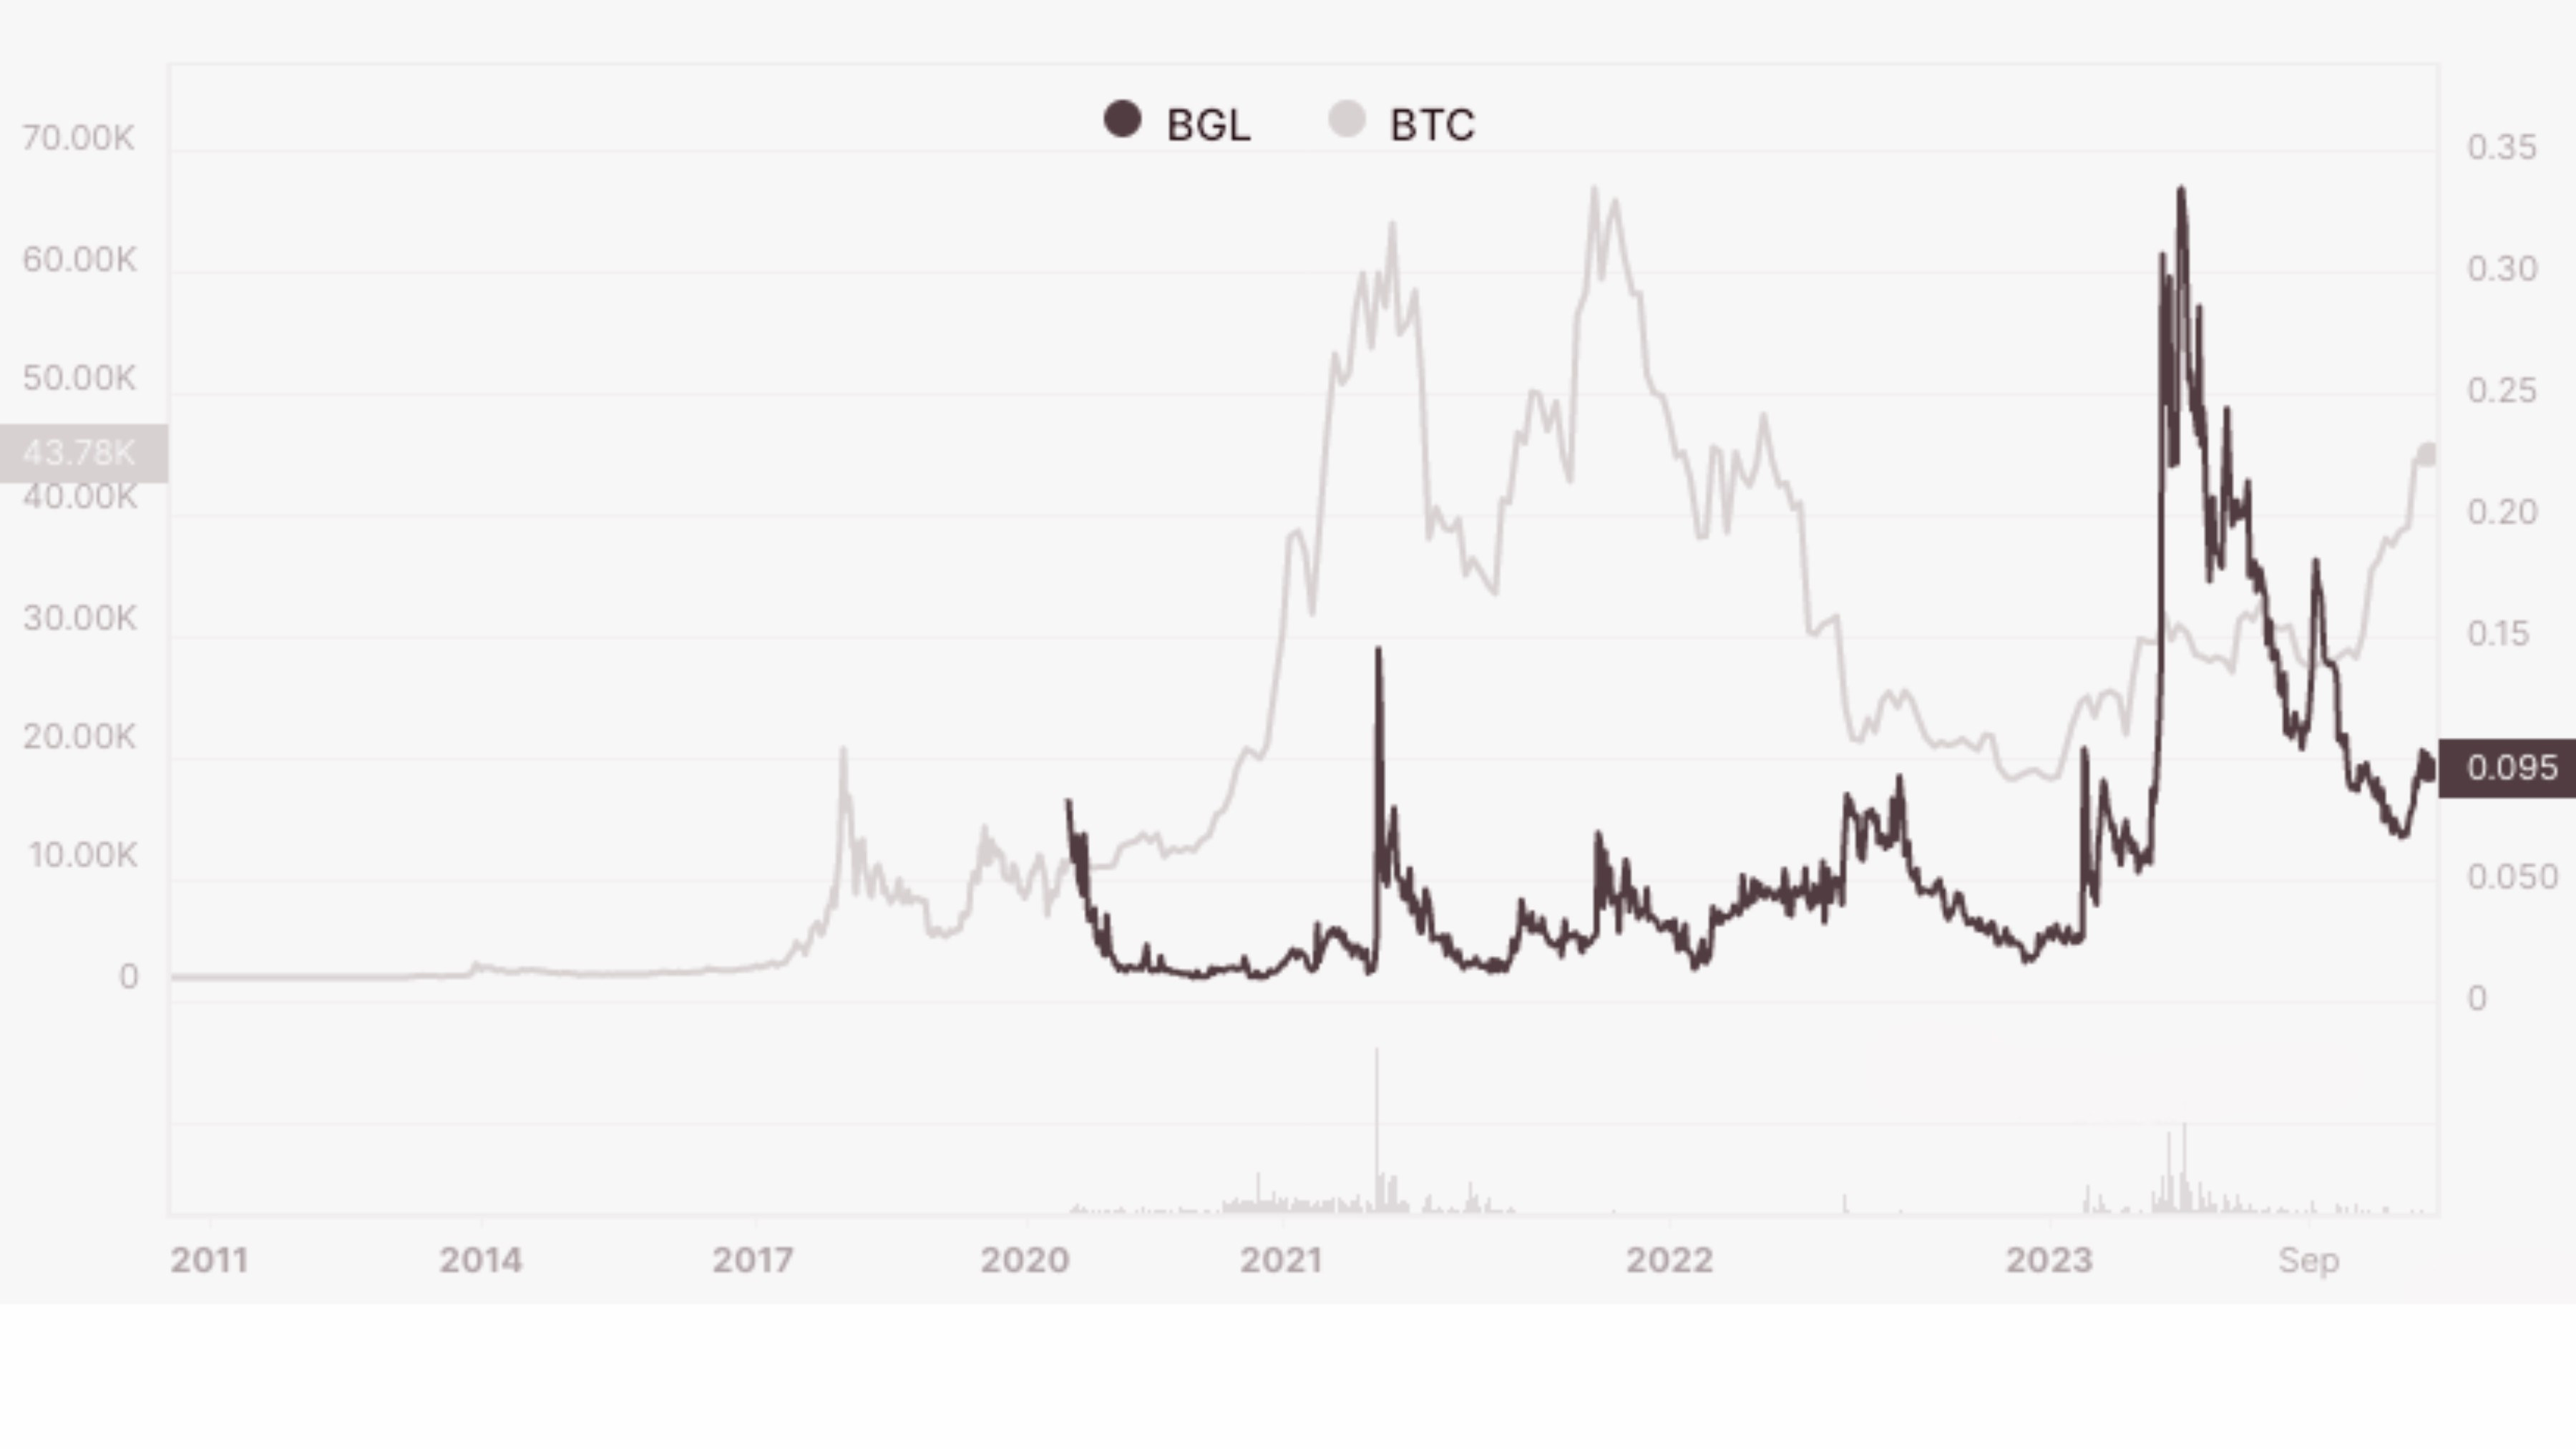
\includegraphics[scale=0.24]{image04.png}}

The insurance capital asset chosen was BGL (Bitgesell). BGL (Bitgesell) is a well-developed fork of Bitcoin with many parameters that remain the same, such as limited supply (21 million), but with the additional mechanics of burning 90\% of the transaction fees and having block reward halving every year. It is running on its own blockchain, which is very similar to Bitcoin. The reasons for selecting BGL as a part of collateral are:

\begin{itemize}
	\item Based on a proven code with similar blockchain safety as Bitcoin
	\item More coin scarcity in the long run compared to Bitcoin
	\item Small market cap that has significant upside potential
\end{itemize}


\subsection{ICT tokens}

By contributing BGL (WBGL in BEP20, ERC20) to the insurance capital, users can mint ICT (Insurance Capital Treasures). The minting of ICT will follow these progression ratios:

\begin{enumerate}
    \item Initially, 1 ICT can be minted for 1 WBGL during the first 3 months after deployment.
    \item Subsequently, every 3 months, the exchange rate of ICT will increase by 1.
    \item The progression will stop increasing when the ratio reaches 10 WBGL for 1 ICT.
\end{enumerate}

This progression was selected to ensure a fair distribution of ICT tokens, particularly benefiting valuable contributors to the insurance capital at the project's early stage.


\subsection{Risk-reward for ICT token holders}

USSD's main focus is on security. Those who value security can play a role in providing it and, in return, get rewarded for their contribution.

The reward system for ICT token holders activates automatically when the Collateral Ratio reaches a level of 1.05. These rewards are paid as interest to ICT holders. To claim these interests, ICT holders need to stake their ICT in a smart contract.

The interest is calculated at a rate of 4.2\% per year based on the Collateral market value. It is paid through the creation of new USSD tokens every 24 hours, at a daily rate of approximately 0.011507\% (4.2\%/365). The distribution of interests is based on the proportion of staking shares held by ICT holders.

For example, if a total of 500 ICT were minted, and 400 were staked for claiming interests, with David staking 100 ICT, his interest share would be 25\% (100/400).

ICT holders can claim their interests by using a claim reward function at any time.


\subsection{Anti-inflation mechanism for USSD holders}

To protect funds from centralization issues and inflation, an anti-inflation mechanism has been introduced in USSD. USSD users can stake their USSD tokens to receive a share of the interests.

Similar to the reward system, the interest for USSD holders will be automatically activated when the Collateral Ratio reaches the 1.05 level. These interests will be paid to USSD holders and can be claimed by staking USSD in the smart contract.

The interest is calculated as 1.8\% annually based on the Collateral market value. It is paid through the minting of new USSD every 24 hours, using a simple percentage of 1.8\%/365 (or approximately ~0.0049315\% per day). The interests will be distributed according to the staking shares of USSD.

For example, if a total of 3,500,000 USSD were minted, with 500,000 were staked for claiming interests, and David had staked 100,000 USSD, his interest share would be 20\% (100,000/500,000). If the collateral ratio of the main collateral is 150\%, overall interests income will be 94,500 USSD (3,500,000 * 150\% * 1,8\%).

David's interests share will be 18 900 USSD (94,500 * 20\%) or 18.9\% interests Annual Percentage Yield (APY) would (18,900/100,000).


\subsection{Risk management mechanisms}


\subsubsection{Wrapped token centralization risks}

Before a trusted and time-proven decentralized bridge is developed, every wrapped token carries centralization risks. Due to various ways the owner can manipulate the smart contract of the wrapped token, manual and limited defense mechanisms were implemented in USSD:

\begin{enumerate}
	\item The USSD owner can change the stable coin to another stable coin once. For example, in the BEP20 contract, the USSD contract owner can change BSC-USD stable coin to DAI (0x1af3f329e8be154074d8769d1ffa4ee058b1dbc3).
	\item The USSD owner can remove stable coins from the collateral structure once. In this case, USSD will be backed only by BTC and ETH.
	\item The USSD owner can switch the insurance capital coin from wBGL to ETH once.
\end{enumerate}

\subsubsection{Bank run protection mechanism}

A "bank run" is like a panic game that happens when a stable coin doesn't have enough collateral. This means there's a chance you might be late in getting your money back from the stablecoin, and the best strategy is to withdraw as much as possible.

To stop this scenario, a feature called "proportional redeem" was added. This lets users who don't want to wait for the collateral value to recover redeem their collateral in proportion to the collateral ratio, thus, protecting other users who do not want to redeem at the moment, and penalizing panic participants.
For example, if the collateral ratio falls to 98\%, USSD holders can redeem 1 USSD for \$0.98 worth of assets.

If the collateral ratio falls below 95\%, those who don't want to take any risks connected to the collateral and want to redeem will get USSD with a 5\% discount.

For instance, if the collateral ratio falls to 93\%, USSD holders can redeem 1 USSD for \$0.884 (93\% * (100\% - 5\%)).

\subsection{Insurance case scenario}

If the rate drops below 90\%, the insurance capital will start distributing funds to the main collateral. This means that every 24 hours, 1\% of assets from the insurance capital contract will be moved to the main collateral (until it reaches 90\% again).

